%%%%%%%%%%%%%%%%%%%%%%%%%%%%%%%%%%%%

\section{確率の定義}

%%%%%%%%%%%%%%%%%%%%%%%%%%%%%%%%%%%%

\subsection{確率}

%%%%%%%%%%%%%%%%%%%%%%%%%%%%%%%%%%%%

\begin{frame}
\frametitle{確率的プロセス}

\twocol{0.5}{0.5}
{
\begin{itemize}

\item \hl{確率的プロセス}とは、何が起こりうるかはわかっているが、実際にどの結果が起こるかわからない状況のことである。

\item 例：コイン投げ、サイコロの目、iTunes シャッフル、明日の株式市場の上下など。

\item 実際には確率的でなくても、プロセスを確率的にモデル化することが有用な場合がある。

\end{itemize}
}{
\begin{center}
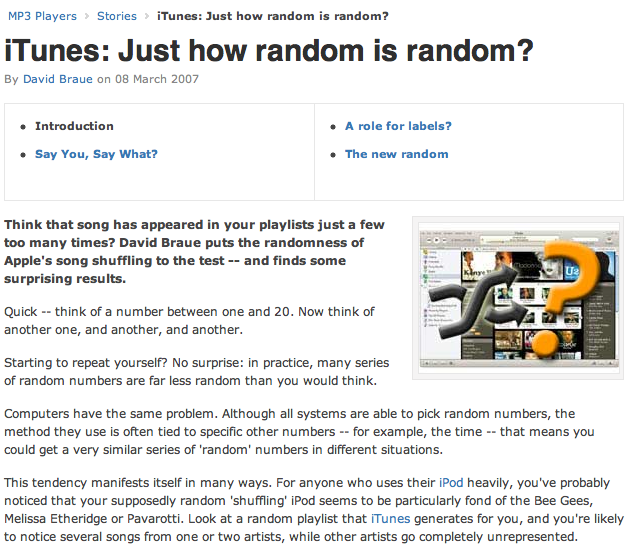
\includegraphics[width=\textwidth]{3-1_define_probability/figures/iTunes}
\end{center}
\ct{ \webURL{http://www.cnet.com.au/itunes-just-how-random-is-random-339274094.htm}}
}

\end{frame}

%%%%%%%%%%%%%%%%%%%%%%%%%%%%%%%%%%%%

\begin{frame}
\frametitle{確率}

\begin{itemize}

\item 確率にはいくつかの解釈があるが、確率が従うべき数学的規則についてはほぼ完全に一致している。
\begin{itemize}
\item $P(A)$ = 事象 A の確率
\item $0 \le P(A) \le 1$
\end{itemize}

\item \hl{頻度論的解釈：}
\begin{itemize}
\item ある結果の確率は、確率的プロセスを無限回観察したときにその結果が起こる割合である。
\end{itemize}

\item \hl{ベイズ的解釈：}
\begin{itemize}
\item ベイズ主義者は確率を主観的な信念の度合いとして解釈する：同じ事象でも、異なる人が異なる確率を割り当てることがある。
\item 過去20年間の計算技術と方法の革命的進歩によって広まった。
\end{itemize}

\end{itemize}

\end{frame}

%%%%%%%%%%%%%%%%%%%%%%%%%%%%%%%%%%%%

\begin{frame}[shrink=25]
\frametitle{練習問題}

\pq{次のどの事象が最も驚くべきものか？}

\begin{enumerate}[(a)]
\item 10回コインを投げて、ちょうど3回表が出る
\item 100回コインを投げて、ちょうど3回表が出る
\solnMult{1000回コインを投げて、ちょうど3回表が出る}
\end{enumerate}

\end{frame}

%%%%%%%%%%%%%%%%%%%%%%%%%%%%%%%%%%%%

\begin{frame}
\frametitle{大数の法則}

\hl{大数の法則}とは、観測数が増えるにつれて、ある特定の結果が起こる割合 \mathhl{\hat{p}_n} が、その結果の確率 \mathhl{p} に収束することを述べたものである。

\end{frame}

%%%%%%%%%%%%%%%%%%%%%%%%%%%%%%%%%%%%

\begin{frame}[shrink=15]
\frametitle{大数の法則（続き）}

\dq{\textit{公正な}コインを投げたとき、最初の10回すべてで表が出た場合、次の投げで表が出る確率はいくつだと思うか？ 0.5、0.5より小さい、それとも0.5より大きい？}

\[ \underline{H} \hspace{1mm} \underline{H} \hspace{1mm} \underline{H} \hspace{1mm} \underline{H} \hspace{1mm} \underline{H} \hspace{1mm} \underline{H} \hspace{1mm} \underline{H} \hspace{1mm} \underline{H} \hspace{1mm} \underline{H} \hspace{1mm} \underline{H} \hspace{1mm} \underline{?} \]

\begin{itemize}
\item 確率はやはり 0.5 であり、次の投げで表が出る確率は 50\% である。
\[ P(H \text{ on 11}^{th} \text{ toss}) = P(T \text{ on 11}^{th} \text{ toss}) = 0.5 \]
\item コインは「裏を出すべき」ではない。
\item 大数の法則についての一般的な誤解は、確率的プロセスは過去に起こったことを補正するはずだというものであるが、これは誤りであり、\hl{ギャンブラーの誤謬}（または\hl{平均の法則}）とも呼ばれる。
\end{itemize}

\end{frame}

%%%%%%%%%%%%%%%%%%%%%%%%%%%%%%%%%%%%

\subsection{互いに排反な結果}

%%%%%%%%%%%%%%%%%%%%%%%%%%%%%%%%%%%%

\begin{frame}[shrink=10]
\frametitle{互いに排反な結果とそうでない結果}

\hl{互いに排反（mutually exclusive）な結果：}同時には起こり得ない。
\begin{itemize}
\item 1回のコイン投げの結果が表と裏の両方になることはない。
\item 学生が同じ科目で合格と不合格の両方になることはない。
\item 1枚のカードがエースとクイーンの両方であることはない。
\end{itemize}

\hl{互いに排反でない結果：}同時に起こり得る。
\begin{itemize}
\item 学生が同じ学期に統計学でA、経済学でAをとることがある。
\end{itemize}

\end{frame}

%%%%%%%%%%%%%%%%%%%%%%%%%%%%%%%%%%%%

\begin{frame}[shrink=10]
\frametitle{互いに排反でない事象の和事象}

\dq{よくシャッフルされた1組のトランプから、ジャックまたは赤いカードを引く確率は何か？}

\begin{figure}
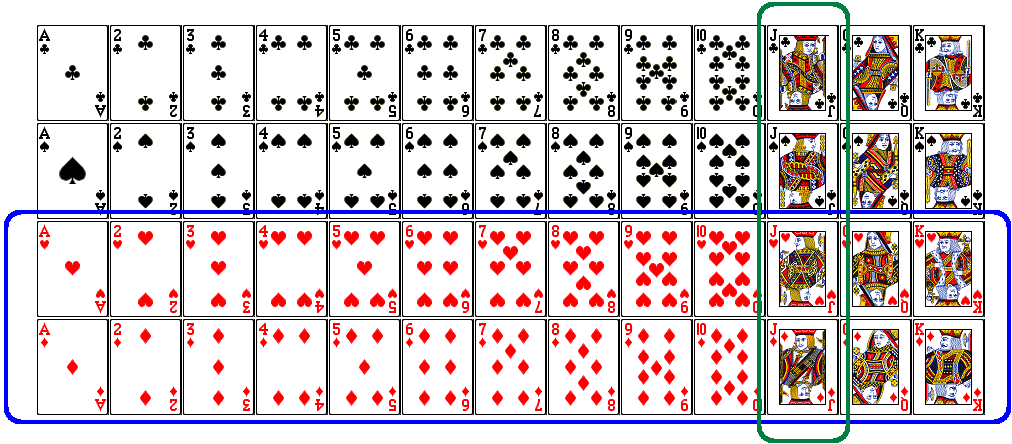
\includegraphics[width=0.7\textwidth]{3-1_define_probability/figures/cards}
\end{figure}

\vspace{-0.75cm}

\soln{
\begin{align*}
P(\text{ジャックまたは赤}) &= P(\text{ジャック}) + P(\text{赤}) - \orange{$P(\text{ジャックかつ赤})$} \\
&= \frac{4}{52} + \frac{26}{52} - \frac{2}{52} = \frac{28}{52}
\end{align*}
}

\vfill

\ct{Figure from \webURL{http://www.milefoot.com/math/discrete/counting/cardfreq.htm}.}

\end{frame}

%%%%%%%%%%%%%%%%%%%%%%%%%%%%%%%%%%%%

\subsection{事象が互いに排反でない場合の確率}

%%%%%%%%%%%%%%%%%%%%%%%%%%%%%%%%%%%%

\begin{frame}
\frametitle{練習問題}

\pq{無作為に選ばれた学生が、大麻を合法化すべきと考えている\underline{か}、または親の政治的見解に同意している確率は何か？}

{\small
\begin{center}
\begin{tabular}{l  cc c}
            & \multicolumn{2}{c}{\textit{親の政治観に同意}} & \\
\cline{2-3}
\textit{大麻合法化} & なし & あり & 合計 \\
\hline
反対          & 11 & 40 & 51 \\
賛成         & 36 & 78 & 114 \\
\hline
合計       & 47 & 118 & 165
\end{tabular}
\end{center}
}

\begin{enumerate}[(a)]
\item $\frac{40 + 36 - 78}{165}$
\solnMult{$\frac{114 + 118 - 78}{165}$}
\item $\frac{78}{165}$
\item $\frac{78}{188}$
\item $\frac{11}{47}$
\end{enumerate}

\end{frame}

%%%%%%%%%%%%%%%%%%%%%%%%%%%%%%%%%%%%

\begin{frame}
\frametitle{まとめ}

\formula{一般加法定則}{\[ P(A~\text{または}~B) = P(A) + P(B) - P(A~\text{かつ}~B) \]}

\Note{互いに排反な事象では $P(A~\text{かつ}~B) = 0$ なので、上式は $P(A~\text{または}~B) = P(A) + P(B)$ に簡略化される。}

\end{frame}

%%%%%%%%%%%%%%%%%%%%%%%%%%%%%%%%%%%%

\subsection{確率分布}

%%%%%%%%%%%%%%%%%%%%%%%%%%%%%%%%%%%%

\begin{frame}
\frametitle{確率分布}

\hl{確率分布}は、起こりうるすべての事象とそれらが起こる確率を一覧にしたものである。

\begin{itemize}
\item 1人の子どもの性別の確率分布：
{\footnotesize
\begin{center}
\begin{tabular}{r | c | c}
事象    & 男		& 女 \\
\hline
確率	& 0.5		& 0.5 \\
\end{tabular}
\end{center}
}

\item 確率分布の規則：
\begin{enumerate}
\item 列挙された事象は互いに排反でなければならない
\item 各確率は0以上1以下でなければならない
\item 確率の合計は1でなければならない
\end{enumerate}

\item 2人の子どもの性別の確率分布：
\soln{
{\footnotesize
\begin{center}
\begin{tabular}{r | c | c | c | c}
事象		& MM	& FF		& MF		& FM \\
\hline
確率	& 0.25	& 0.25	& 0.25	& 0.25 \\
\end{tabular}
\end{center}
}}

\end{itemize}

\end{frame}

%%%%%%%%%%%%%%%%%%%%%%%%%%%%%%%%%%%%

\begin{frame}
\frametitle{練習問題}

\pq{調査で、回答者の52\%が民主党員だと答えた。このサンプルから無作為に選ばれた回答者が共和党員である確率はいくつか？}

\begin{enumerate}[(a)]
\item 0.48
\item 0.48より大きい
\item 0.48より小さい
\solnMult{与えられた情報だけでは計算できない}
\end{enumerate}

\only<2->{\orange{唯一の2つの政党が共和党と民主党である場合は (a) が可能である。しかし、政党に所属しない人やこれら2つ以外の政党に所属する人もいる可能性があるため、(c) も可能である。(b) は合計確率が1を超えることになるため、絶対に不可能である。}}

\end{frame}

%%%%%%%%%%%%%%%%%%%%%%%%%%%%%%%%%%%%

\subsection{余事象}

%%%%%%%%%%%%%%%%%%%%%%%%%%%%%%%%%%%%

\begin{frame}
\frametitle{標本空間と余事象}

\hl{標本空間}は、試行で起こりうるすべての結果の集合である。

\begin{itemize}
\item ある夫婦に1人の子どもがいる場合、その性別の標本空間は？ $S = \{ M, F \}$
\item ある夫婦に2人の子どもがいる場合、その性別の標本空間は？ \soln{$S = \{ MM, FF, FM, MF \}$}
\end{itemize}

\hl{余事象}は、確率の和が1になる2つの互いに排反な事象である。

\begin{itemize}
\item ある夫婦に1人の子どもがいる。その子が男の子でないとわかった場合、その性別は？
\{ \sout{\textcolor{gray}{M}}, \orange{F} \} $\rightarrow$ 男の子と女の子は\hl{余事象}である。
\item ある夫婦に2人の子どもがいる。両方が女の子でないとわかった場合、可能な性別の組み合わせは？
\soln{\{ \orange{MM}, \sout{\textcolor{gray}{FF}}, \orange{FM}, \orange{MF} \} }
\end{itemize}

\end{frame}

%%%%%%%%%%%%%%%%%%%%%%%%%%%%%%%%%%%%

\subsection{独立}

%%%%%%%%%%%%%%%%%%%%%%%%%%%%%%%%%%%%

\begin{frame}
\frametitle{独立}

2つのプロセスが\hl{独立}であるとは、一方の結果を知っても他方の結果についての有用な情報が得られない場合をいう。

\begin{itemize}

\item 最初の投げでコインが表になったことを知っても、2回目の投げでコインがどちらになるかについての有用な情報は得られない。$\rightarrow$ 2回のコイン投げの結果は独立である。

\item 最初に引いたカードがエースであることを知ると、2回目の引きでエースを引く確率についての有用な情報が得られる。$\rightarrow$ デッキからの2回の引き（非復元）の結果は従属である。

\end{itemize}

\end{frame}

%%%%%%%%%%%%%%%%%%%%%%%%%%%%%%%%%%%%

\begin{frame}
\frametitle{練習問題}

\pq{\small{2013年1月9日〜12日、SurveyUSA がノースカロライナ州の居住者500人の無作為標本を対象に、銃の広範な所有は法を守る市民を犯罪から守るか、社会をより危険にするかを質問した。回答者全体の58\%が「市民を守る」と回答した。白人回答者の67\%、黒人回答者の28\%、ヒスパニック回答者の64\%がこの見解を共有していた。次のうち正しいものはどれか？}}

銃所有に関する意見と人種・民族は最も可能性が高いのは
\begin{enumerate}[(a)]
\item 余事象
\item 互いに排反
\item 独立
\solnMult{従属}
\item 互いに排反
\end{enumerate}

\ct{\webURL{http://www.surveyusa.com/client/PollReport.aspx?g=a5f460ef-bba9-484b-8579-1101ea26421b}}

\end{frame}

%%%%%%%%%%%%%%%%%%%%%%%%%%%%%%%%%%%%

\begin{frame}[shrink=15]
\frametitle{}

\formula{独立性の確認}{P(B が真であるとき A が起こる) = $P(A~|~B) = P(A)$ ならば、A と B は独立である。}

$\:$ \\

\soln{P(市民を守る) = 0.58 \\
$\:$ \\
P(無作為に選ばれたノースカロライナ州居住者が銃所有は市民を守ると答える，その居住者が白人である場合) = \\ P(市民を守る $|$ 白人) = 0.67 \\
$\:$ \\
P(市民を守る $|$ 黒人) = 0.28 \\
$\:$ \\
P(市民を守る $|$ ヒスパニック) = 0.64 \\
$\:$ \\
P(市民を守る) は人種・民族によって異なるため、銃所有に関する意見と人種・民族は最も可能性が高いのは従属である。
}

\end{frame}

%%%%%%%%%%%%%%%%%%%%%%%%%%%%%%%%%%%%

\begin{frame}[shrink=10]
\frametitle{標本データに基づく従属性の判定}

\begin{itemize}

\item 標本データから計算された条件付き確率が2つの変数間の従属性を示している場合、次のステップは、確率の観測された差が偶然に起こる可能性があるかを判定する仮説検定を行うことである。

\item 条件付き確率間の観測された差が大きいほど、その差が真であるという証拠が強くなる。

\item 標本が大きい場合、小さな差でも真の差の強い証拠となりうる。

\end{itemize}

\dq{{\small P(市民を守る $|$ 白人) = 0.67、P(市民を守る $|$ ヒスパニック) = 0.64 であった。白人とヒスパニックで銃の広範な所有が市民を守ると思う割合に真の差があると確信するのはどちらの条件下か？ $n = 500$ か $n = 50,000$ か？}} \soln{$n = 50,000$}

\end{frame}

%%%%%%%%%%%%%%%%%%%%%%%%%%%%%%%%%%%%

\begin{frame}
\frametitle{}

\formula{独立事象の積の法則}{\[P(A~\text{かつ}~B) = P(A) \times P(B) \]
\small{より一般的には、$P(A_1~\text{かつ}~\cdots~\text{かつ}~A_k) = P(A_1) \times \cdots \times P(A_k)$}}

\dq{コインを2回投げるとき、2回続けて裏が出る確率は何か？}

\[ P(\text{1回目に裏}) \times  P(\text{2回目に裏}) = \frac{1}{2} \times \frac{1}{2} = \frac{1}{4} \]

\end{frame}

%%%%%%%%%%%%%%%%%%%%%%%%%%%%%%%%%%%%

\begin{frame}[shrink=10]
\frametitle{練習問題}

\pq{最近のギャラップ調査によると、2012年6月時点でテキサス州民の25.5\%が健康保険を持っていない。非加入率が一定であると仮定して、無作為に選んだ2人のテキサス州民が両方とも非加入である確率は何か？}

\twocol{0.4}{0.6}
{
\begin{enumerate}[(a)]
\item $25.5^2$
\solnMult{$0.255^2$}
\item $0.255 \times 2$
\item $(1 - 0.255)^2$
\end{enumerate}
}
{
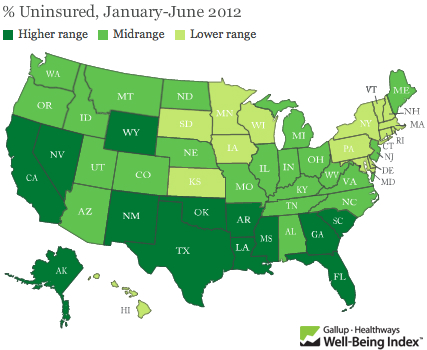
\includegraphics[width=0.9\textwidth]{3-1_define_probability/figures/uninsured}
}

\ct{ \webURL{http://www.gallup.com/poll/156851/uninsured-rate-stable-across-states-far-2012.aspx}}

\end{frame}

%%%%%%%%%%%%%%%%%%%%%%%%%%%%%%%%%%%%

\subsection{まとめ}

%%%%%%%%%%%%%%%%%%%%%%%%%%%%%%%%%%%%

\begin{frame}
\frametitle{互いに排反 vs. 余事象}

\dq{2つの互いに排反な事象の確率の和は常に1になるか？}

\soln{必ずしもそうではない。標本空間に3つ以上の事象がある場合がある（例：党派）。}

$\:$ \\

\dq{2つの余事象の確率の和は常に1になるか？}

\soln{はい、それが余事象の定義である（例：表と裏）。}

\end{frame}

%%%%%%%%%%%%%%%%%%%%%%%%%%%%%%%%%%%%

\begin{frame}
\frametitle{すべてをまとめると…}

\dq{テキサス州民を5人無作為に選ぶとき、少なくとも1人が保険未加入である確率は何か？}

\begin{itemize}

\item テキサス州民を5人無作為に選んだ場合、保険未加入者の人数の標本空間は：
\[ S = \{0, 1, 2, 3, 4, 5\} \]

\item 少なくとも1人が保険未加入である場合に注目する：
\[ S = \{0, \orange{$1, 2, 3, 4, 5$} \} \]

\item 標本空間を2つのカテゴリに分割できる：
\[ S = \{0, \orange{\text{少なくとも1人}} \} \]

\end{itemize}

\end{frame}

%%%%%%%%%%%%%%%%%%%%%%%%%%%%%%%%%%%%

\begin{frame}[shrink=10]
\frametitle{すべてをまとめると…}

標本空間の確率の和は1でなければならないため：
\begin{eqnarray*}
P(\text{少なくとも1人が未加入}) &=& 1 - P(\text{未加入者なし}) \\
&=& 1 - [(1-0.255)^5] \\
&=& 1- 0.745^5 \\
&=& 1 - 0.23 \\
&=& 0.77
\end{eqnarray*}

$\:$ \\
$\:$ \\

\formula{少なくとも1}{\[P(\text{少なくとも1}) = 1 - P(\text{1つもない})\]}

\end{frame}

%%%%%%%%%%%%%%%%%%%%%%%%%%%%%%%%%%%%

\begin{frame}
\frametitle{練習問題}

\pq{ある大学の学部生の約20\%がベジタリアンまたはビーガンである。学部生3人の無作為標本から、少なくとも1人がベジタリアンまたはビーガンである確率は何か？}

\twocol{0.3}{0.6}{
\begin{enumerate}[(a)]
\item $1 - 0.2 \times 3$
\item $1 - 0.2^3$
\item $0.8^3$
\item $1 - 0.8 \times 3$
\solnMult{$1 - 0.8^3$}
\end{enumerate}
}
{
\soln{
$P(\text{少なくとも1人がベジタリアン}) = 1- P(\text{ベジタリアンなし})$ \\
$= 1 - (1 - 0.2)^3$ \\
$= 1 - 0.8^3$ \\
$= 1 - 0.512 = 0.488$ }
}

\end{frame}

%%%%%%%%%%%%%%%%%%%%%%%%%%%%%%%%%%%%
